% kapitel2.tex
%\chapter{Die Softwarekonstruktion}
%\label{chapter:kap2}
\section{Aufbau der Softwarearchitektur}
Wie im ersten Teil der Ausarbeitung verdeutlicht wurde, ist der Raspberry Pi im Inneren des Spiegels das Kernstück der gesamten Plattform. Auf dieser Hardwarekomponente läuft dementsprechend die komplett entwickelte Software. 

Das Softwareprojekt selbst ist in zwei Komponenten aufgeteilt. Die erste Softwarekomponente realisiert die eigentliche SmartMirror-Anwendung inklusive der Ausgestaltung der Benutzungsschnittstelle, der Kommunikation mit verbauten Sensoren und des Datenimportes aus Datenquellen des Internets. Diese Anwendung ist in Python geschrieben, realisiert die SmartMirror-Funktionalität und hat den größten Anteil des Implementierungsaufwandes erfordert. Im Gegensatz dazu steht die zweite Softwarekomponente, im folgenden StartUp-Anwendung genannt, die ein Skript umfasst, das nach dem Systemstart die SmartMirror-Anwendung startet. Bei dieser handelt es sich eher um eine erforderliche Hilfskomponente von geringerem Umfang, die als Bash-Skript direkt ausführbar auf Betriebssystemebene realisiert wurde.  

\begin{figure}
	\centering
	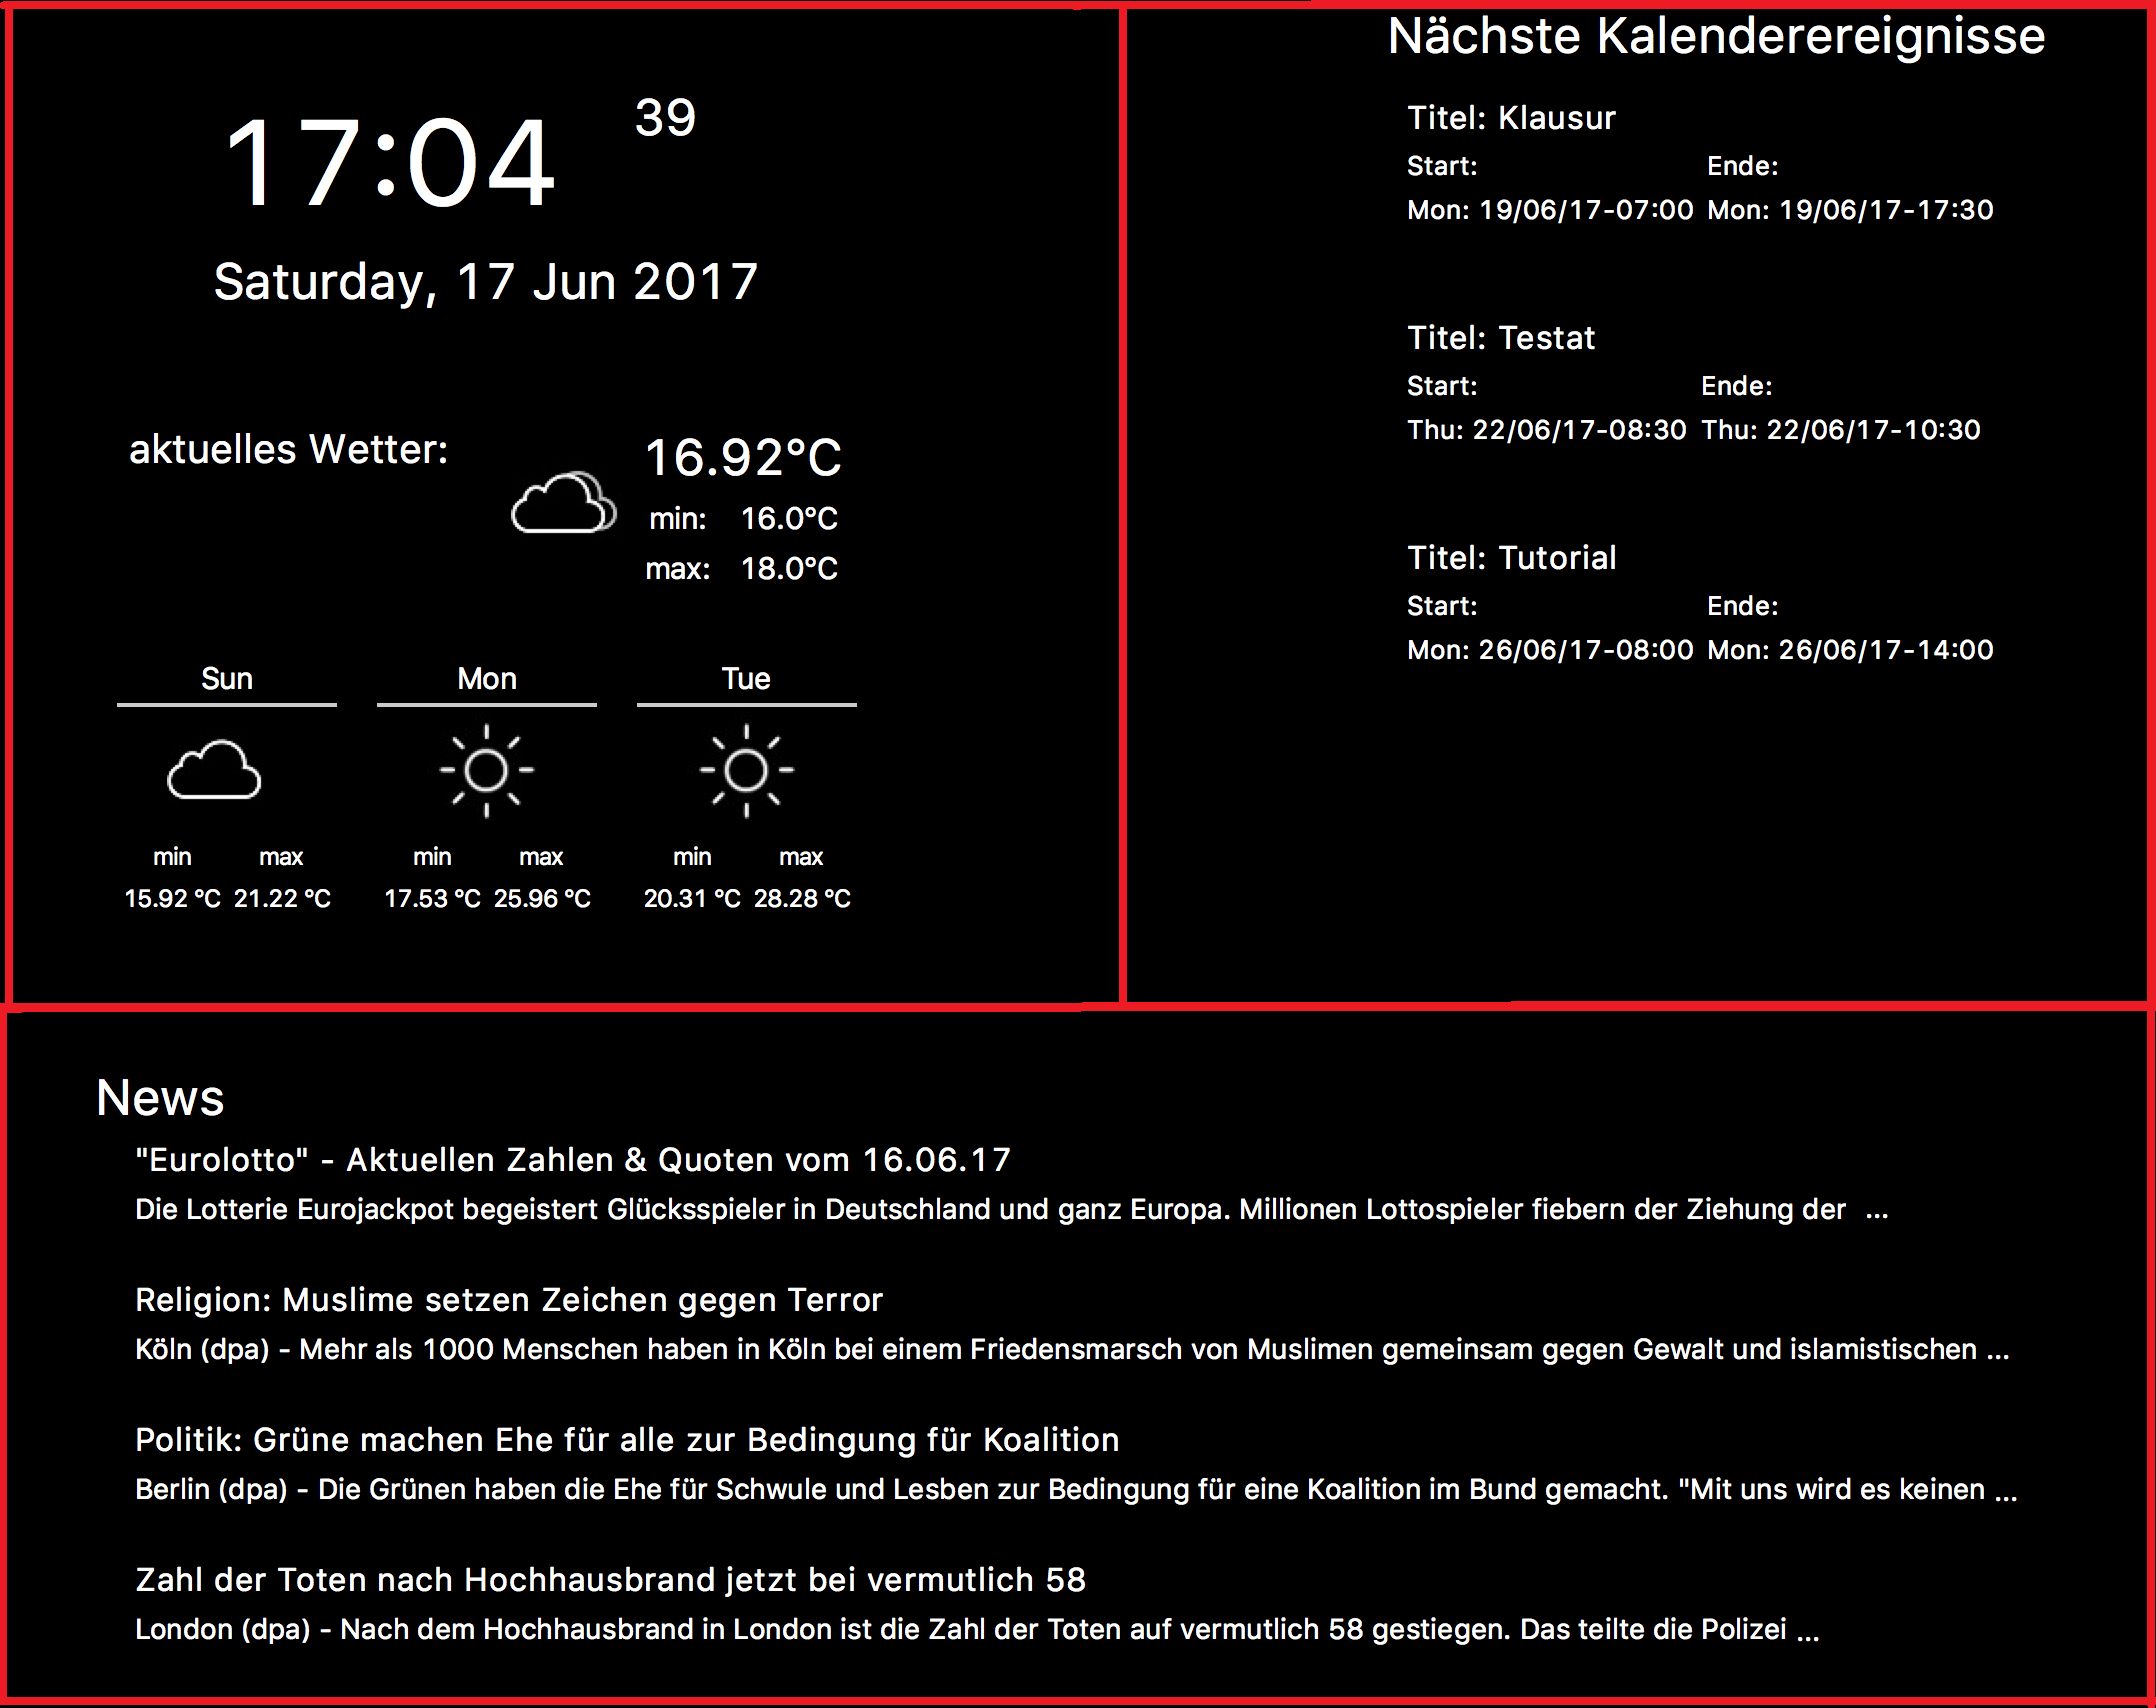
\includegraphics[width=0.7\linewidth]{bilder/grafOberflaeche}
	\caption[Komponentendiagramm der SmartMirror-Applikationen]{Komponentendiagramm der SmartMirror-Applikationen}
	\label{fig:komponentendiagramm}
\end{figure}

Zum besseren Verständnis ist in \autoref{fig:komponentendiagramm} der softwaretechnische Technologiestack der beiden Softwarekomponenten in Form eines UML-Komponentendiagramms dargestellt (Literatur). Die zentrale physikalische Ausführungseinheit ist der Raspberry Pi. Dieser kommuniziert über ... mit den drei verbauten Sensoren: dem Bewegungssensor, dem Temperatursensor und dem .... Alle drei Sensoren wurden so gewählt, dass eine Kommunikation über ... möglich ist. Dieses Protokoll lässt sich über die ...-API (Literatur) sehr gut in Phython-Anwendungen einbinden, wie im \autoref{subsec:kommunikation} weiter ausgeführt wird. Des weiteren zeigt das Diagramm, dass zwei weitere Informationsquellen über das Internet, also das http(s)-Protokoll, angebunden werden. Dabei handelt es sich zum Einen um  
einen Newsserver (XYZ-Adresse?!), über den aktuelle Spiegel-Nachrichten über einen RSS-Feed (Literatur) eingebunden werden können und zum Anderen um die Einbindung eines google-Kalenders. Die Kalendereinträge werden über  REST-Webservices (Literatur) im JSON-Format (Literatur/Quelle) abgefragt. 

Die beiden Softwarekomponenten des SmartMirrors laufen auf Basis eines Linux ..., das als Betriebssystem auf dem Rasberry Pi installiert wurde. Die SmartMirror-Anwendung \glqq SmartMirror.??? \grqq ist ein Artefakt, welches durch den Python-Interpreter \glqq XYZ \grqq interpretiert wird. Das StartUp-Skript kann mit dem Kommando \glqq .... \grqq direkt auf dem Betriebssystem ausgeführt werden. 

Beide Softwarekomponenten werden im Folgenden detaillierter beschrieben: zuerst die SmartMirror-Anwendung und dann das StartUp-Skript.




\begin{figure}
	\centering
	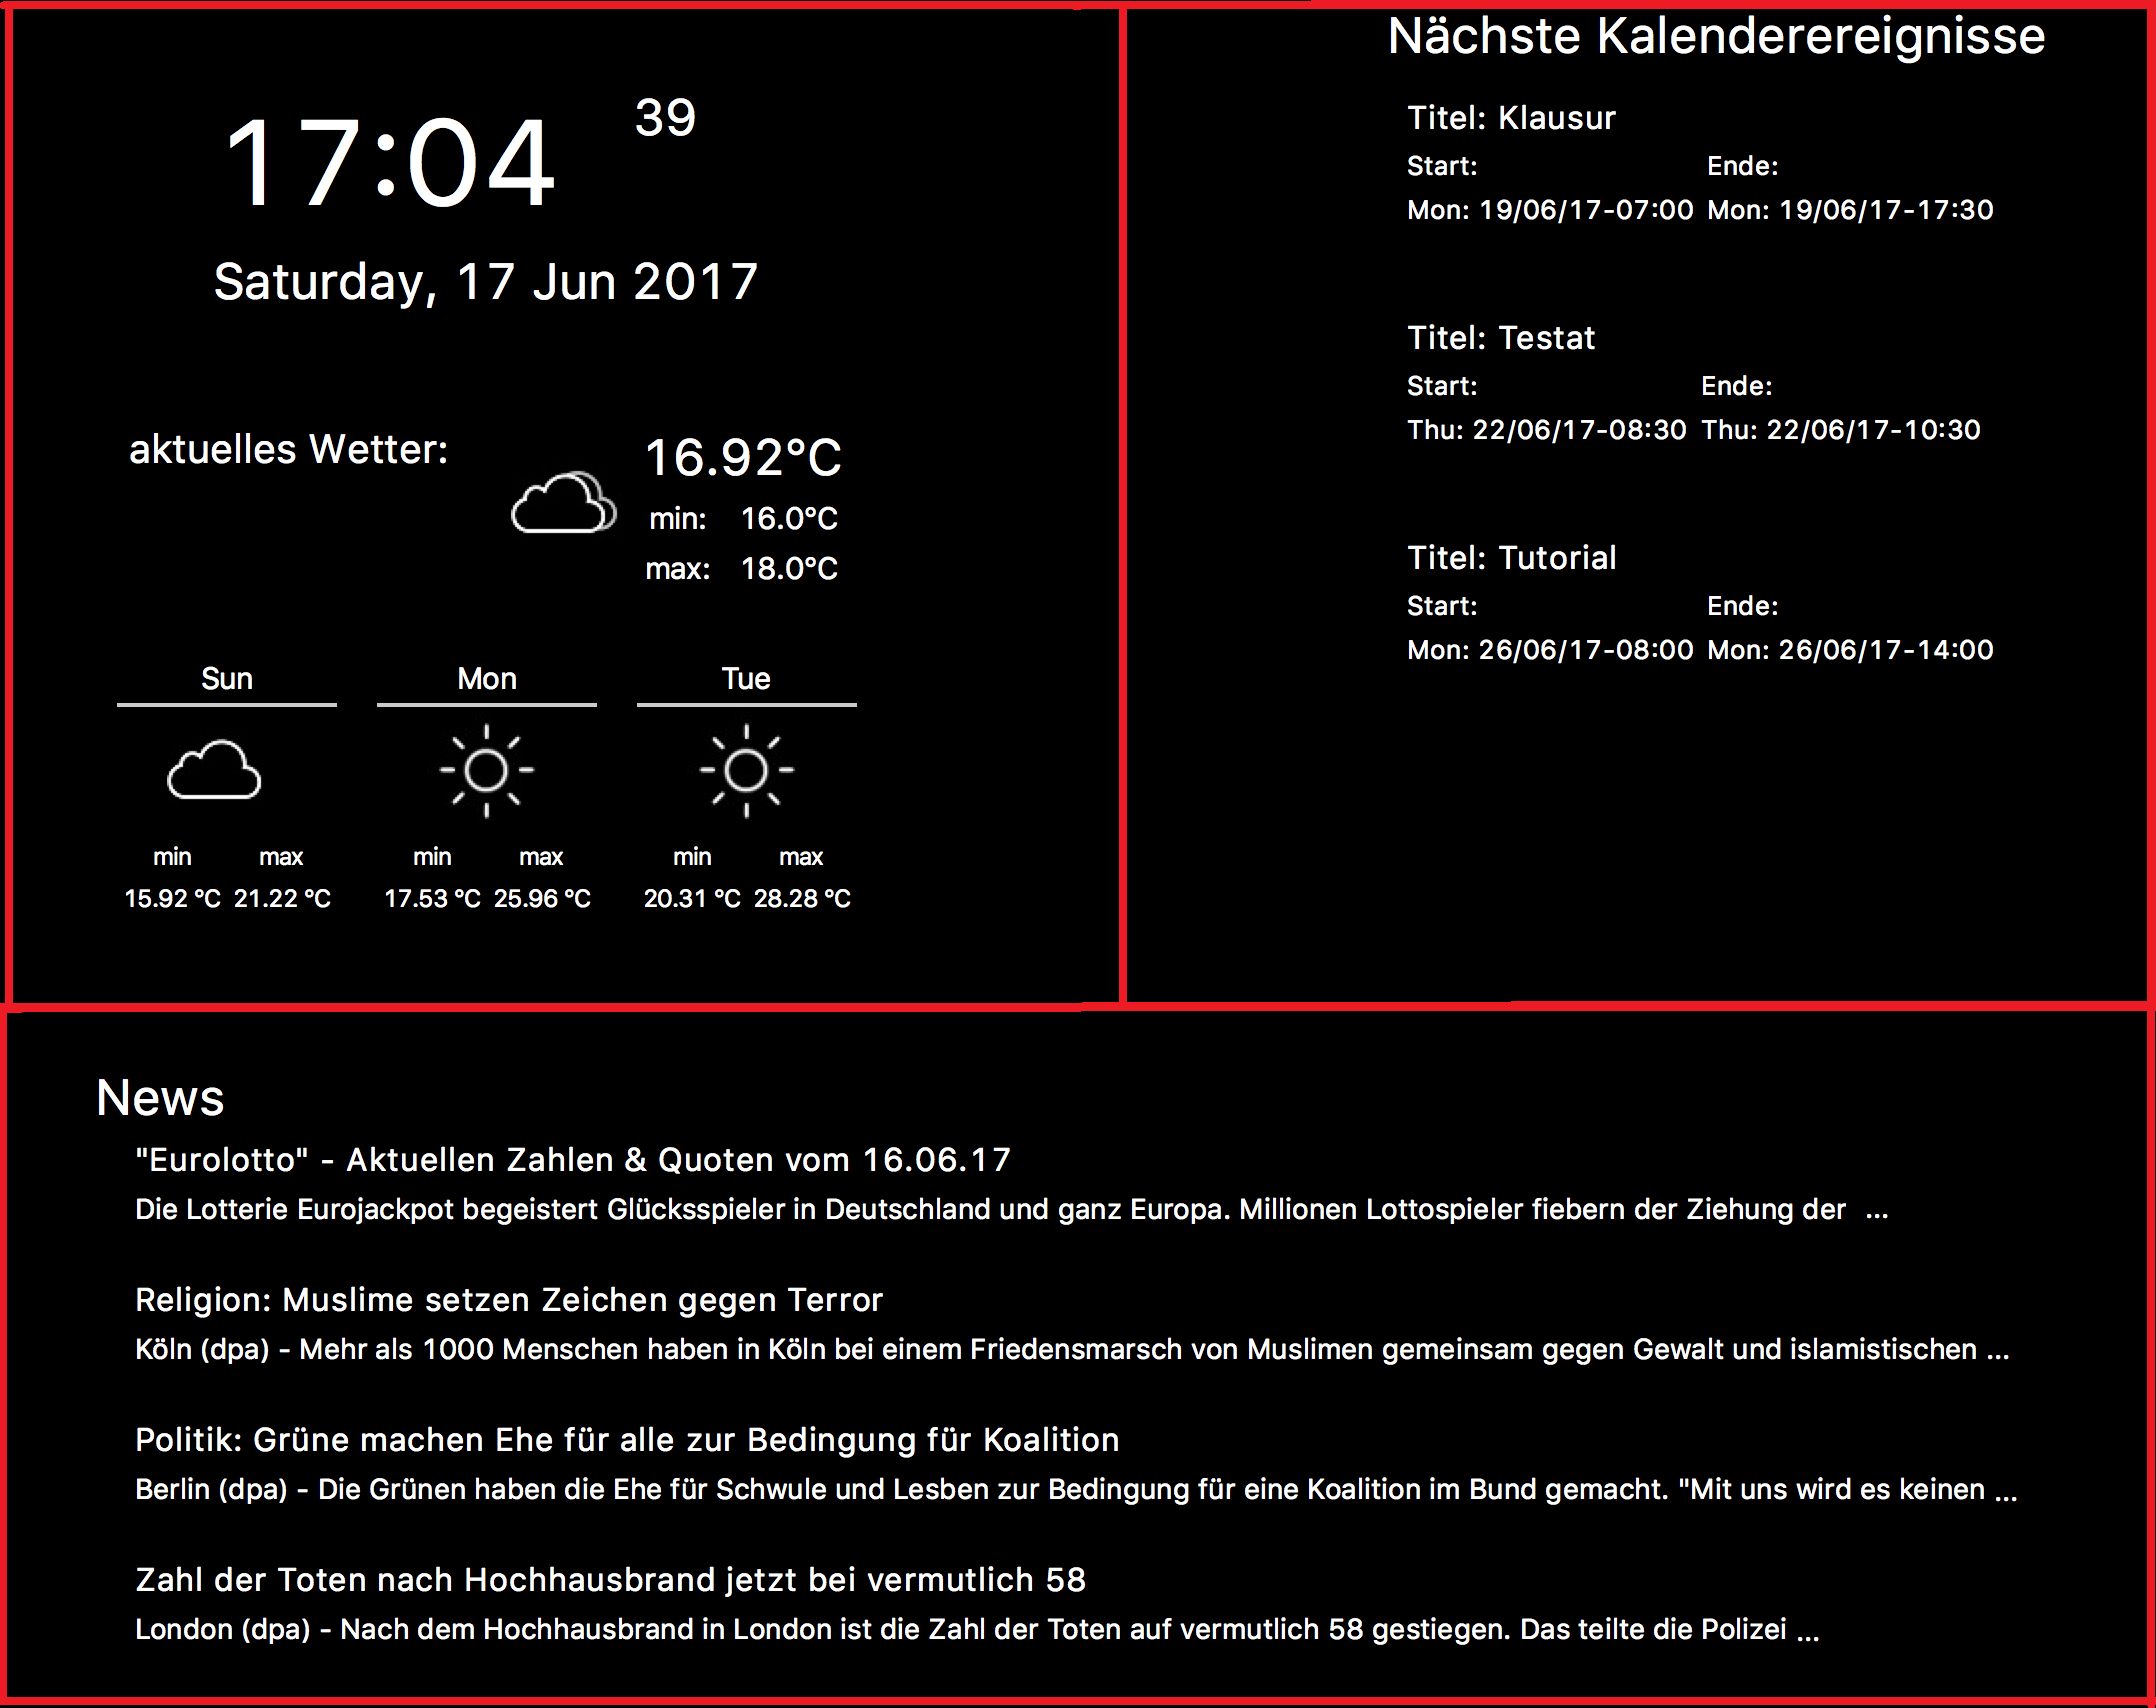
\includegraphics[width=0.7\linewidth]{bilder/grafOberflaeche}
	\caption[UI der SmartMirror Applikation]{UI der SmartMirror Applikation}
	\label{fig:grafoberflaeche}
\end{figure}

\begin{figure}
	\centering
	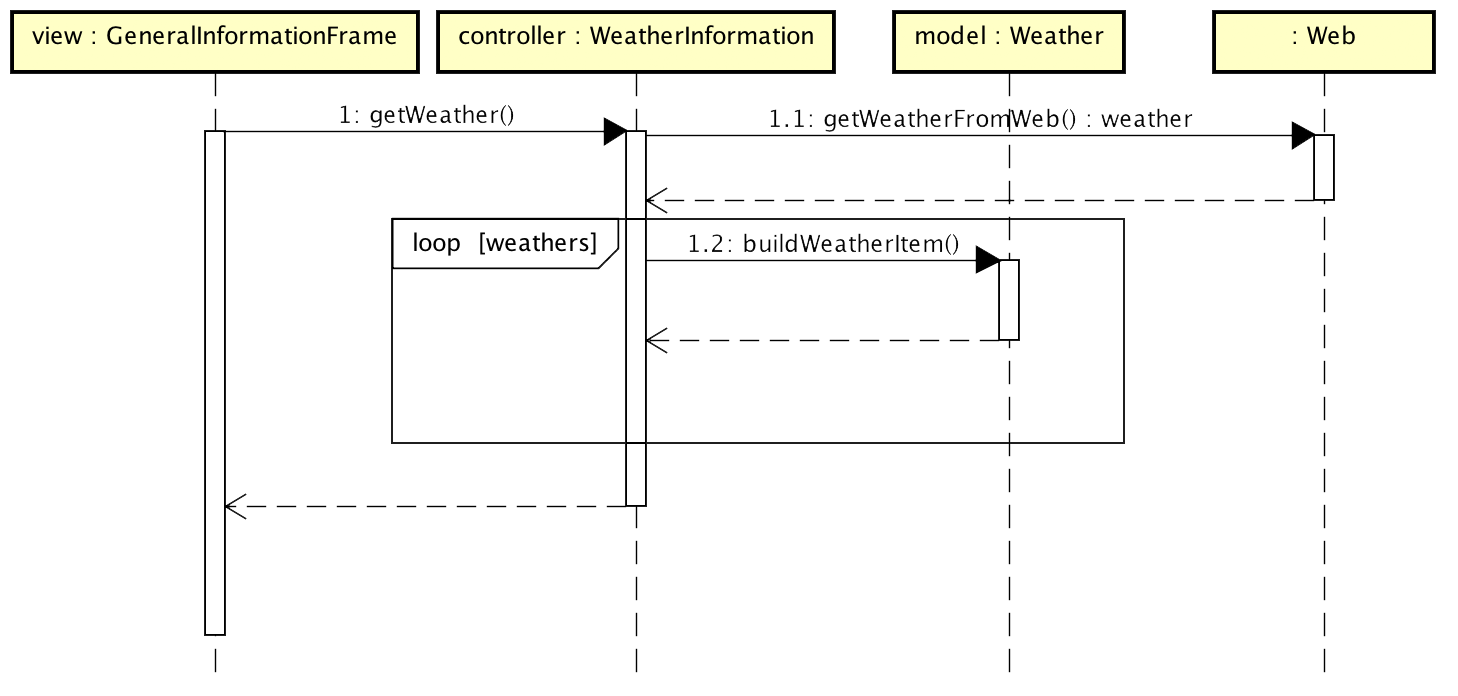
\includegraphics[width=0.7\linewidth]{bilder/sequenceDiagramGettingDataNoBackground}
	\caption{Sequenzdiagramm: Bezug von Daten aus dem Internet}
	\label{fig:sequenzDiagramData}
\end{figure}

\begin{figure}
	\centering
	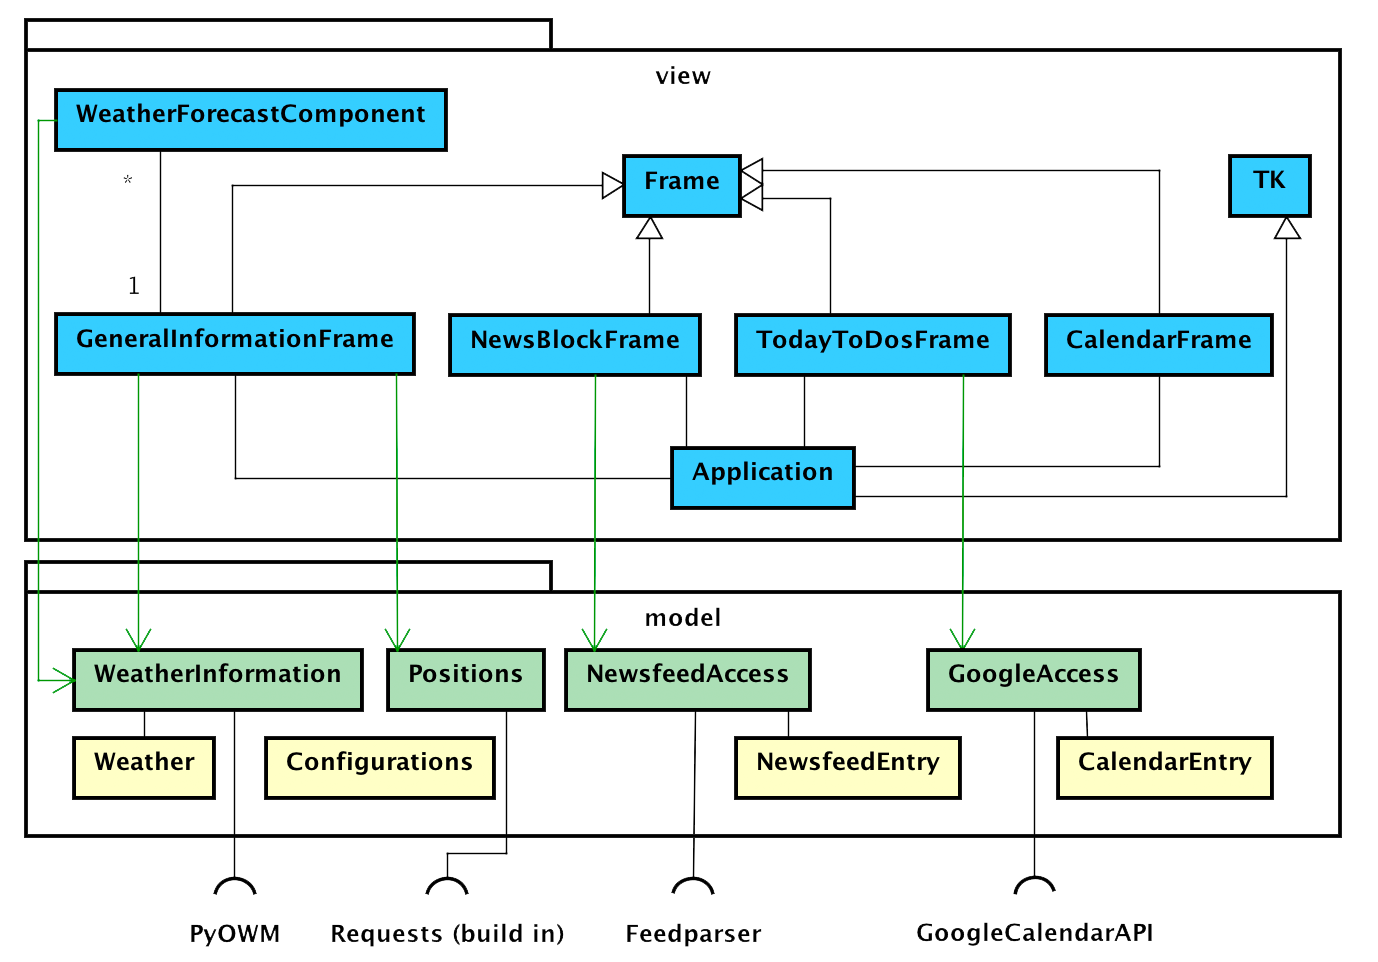
\includegraphics[width=0.7\linewidth]{bilder/umlDiagramNoBackground}
	\caption[UML-Diagramm: Klassenaufbau der Hauptapplikation]{UML-Diagramm: Klassenaufbau der Hauptapplikation}
	\label{fig:umldiagramClasses}
\end{figure}


\subsection{Die SmartMirror-Anwendung}

Die Funktionalität der SmartMirror-Anwendung lässt sich am besten ausgehend von der Gestaltung der Benutzungsschnittstelle erfassen, die in \autoref{fig:grafoberflaeche} dargestellt wird. Die Darstellung lässt sich grob in drei Bereiche strukturieren: den oberen linken Bereich, den oberen rechten und den unteren Bereich. Oben links werden aktuelle Informationen konkret Uhrzeit, Datum und Wetterdaten angezeigt, während im rechten Bereich die nächsten Kalenderereignisse aufgeführt werden und im unteren Bereich aktuelle Neuigkeiten (News) angezeigt werden.





TkInter ... in Python integriert



\subsubsection*{Eingebettete Libraries}

\subsubsection*{Kommunikation mit externen Systemen}
\label{subsec:kommunikation}
\subsubsection*{Aufbau der Anwendung}


\subsection{Das StartUp-Skript}

\section{Der SmartMirror im Einsatz}
\subsection{Inbetriebnahme}
\subsection{Showcase}

\section{Fazit und Ausblick}
